\documentclass[11pt,a4paper]{article}
%\documentclass[onecolumn]{aastex62}
\usepackage[utf8]{inputenc}
\usepackage[T1]{fontenc}      % Mejora la salida de los caracteres acentuados
\usepackage{textcomp} 
\usepackage[spanish]{babel} 

\decimalpoint 
% Creo que queda mejor la versión con punto que con coma

\usepackage{booktabs} % Para líneas horizontales elegantes
\usepackage{siunitx}  % Para alineación decimal y unidades

\setlength{\parskip}{9pt}
\usepackage{graphicx}
\AtBeginDocument{\renewcommand{\contentsname}{Índice}}
\usepackage{changepage}
\usepackage{subcaption}
\usepackage{longtable} 
\usepackage{adjustbox}
\usepackage{array}
\usepackage{setspace}
\usepackage{appendix}
\usepackage{comment}
\usepackage{float}
\usepackage{xcolor}
\usepackage{hyperref}
\definecolor{new_pink}{RGB}{255,20,147} 
\hypersetup{
    colorlinks=true,
    linkcolor=black,
    urlcolor=new_pink  
}
\setstretch{1.15}
% Nuevos tipos de columna para centrado horizontal y vertical
\newcolumntype{C}[1]{>{\centering\arraybackslash}m{#1}}
\newcolumntype{M}[1]{>{\centering\arraybackslash}m{#1}}
\newcolumntype{P}[1]{>{\centering\arraybackslash}m{#1}}
% Nueva columna que combina centrado horizontal y vertical
\newcolumntype{X}[1]{>{\centering\arraybackslash}m{#1}}
%% Tamaño página y máhrgenes
\usepackage[a4paper,top=1.5cm,bottom=2.0cm,left=1.75cm,right=1.75cm,marginparwidth=1.75cm]{geometry}
%\usepackage{dcolumn}% Align table columns on decimal point
%\usepackage{bm}% bold math
\usepackage{amsmath}
\usepackage{amsfonts}
\usepackage{booktabs}
\addto\captionsspanish{\renewcommand{\tablename}{Tabla}}
\addto\captionsspanish{\renewcommand{\lstlistingname}{Código}}

\usepackage{natbib}
% \setcitestyle{numbers}
\bibliographystyle{plainnat}
\usepackage[nottoc]{tocbibind}
\setcitestyle{authoryear}
\newcommand{\Hb}{H$\beta$\xspace}
\newcommand{\Ha}{H$\alpha$\xspace}
\newcommand{\Hd}{H$\delta$\xspace}
\newcommand{\OI}{$\left[\mathrm{O\,\textrm{\sc{i}}}\right]$\xspace}
\newcommand{\SII}{$\left[\mathrm{S\,\textrm{\sc{ii}}}\right]$\xspace}
\newcommand{\OIII}{$\left[\mathrm{O\,\textrm{\sc{iii}}}\right]$\xspace}
\newcommand{\OII}{$\left[\mathrm{O\,\textrm{\sc{ii}}}\right]$\xspace}
\newcommand{\NII}{$\left[\mathrm{N\,\textrm{\sc{ii}}}\right]$\xspace}
\newcommand{\aap}{A\%A}
\newcommand{\vgp}[1]{\textcolor{green}{VGP: #1}}
\newcommand{\lda}[1]{\textcolor{blue}{LDA: #1}}
\newcommand{\jda}[1]{\textcolor{red}{LPF: #1}}
\usepackage{xspace}
\newcommand{\msun}{$h^{-1}{\rm M}_{\odot}$\xspace}
%\usepackage[maxbibnames=3,natbib=true]{biblatex}
 \usepackage{gensymb}
 \usepackage{multirow}

\usepackage{subcaption}
% Macros para revistas (sustituyen a las de RevTeX)
\def\apj{ApJ}
\def\apjl{ApJL}
\def\mnras{MNRAS}
\def\araa{ARA\&A}
\def\aap{A\&A}
\def\prl{Phys.\ Rev.\ Lett.}
\def\prd{Phys.\ Rev.\ D}
\def\icarus{icarus}
\def\aj{Astrophysical Journal}

\usepackage{enumitem}
\setlist[itemize]{label=-}
\usepackage{listings}
\usepackage{hyperref}
\usepackage{amssymb}


% Configuración de bloques de código
\definecolor{codegray}{rgb}{0.95,0.95,0.95}
\definecolor{codegreen}{rgb}{0,0.6,0}
\definecolor{codeblue}{rgb}{0,0,0.6}

\lstdefinestyle{bashstyle}{
    backgroundcolor=\color{codegray},   
    commentstyle=\color{codegreen},
    keywordstyle=\color{blue},
    numberstyle=\tiny\color{gray},
    stringstyle=\color{codeblue},
    basicstyle=\ttfamily\small,
    breakatwhitespace=false,         
    breaklines=true,                 
    captionpos=b,                    
    keepspaces=true,                
    numbers=none,                    
    showspaces=false,                
    showstringspaces=false,
    showtabs=false,                  
    tabsize=2,
    language=python
}

\lstset{style=bashstyle}




\begin{document}
\pagenumbering{arabic}
\onehalfspacing
\begin{center}
{\vspace{2cm}
\textbf{\huge\ Práctica 9: Ecuación de Schrödinger}}\\
\vspace{10pt}
\large
A. López y J. Acebes \hfill Computación Avanzada\hfill 
\end{center}
%%%%%%%%%%%%%%%%%%%%%%%%%%%%%%%%%%

% --- Archivo: sections/1_intro.tex ---
\section{Introducción}

El presente documento aborda el estudio de la dinámica ondulatoria cuántica, escalando desde la fenomenología unidimensional elemental hasta sistemas bidimensionales e interferencia de materia masiva. Inicialmente, se analiza el comportamiento de una partícula cuántica confinada en un pozo de potencial unidimensional con paredes impenetrables en $x=0$ y $x=L$, y su interacción con una barrera de potencial rectangular centrada en $x=x_c<L$. Clásicamente, si la energía cinética es inferior a la altura de la barrera, la transmisión es estrictamente nula. Sin embargo, su naturaleza cuántica y ondulatoria permite una probabilidad no nula de atravesarla, fenómeno conocido como efecto túnel. El objetivo de esta fase es resolver el sistema, visualizar la densidad de probabilidad interactuando con la barrera, y cuantificar las probabilidades de transmisión y reflexión de forma continua así como su dependencia con las características de la barrera.

Posteriormente, el alcance de la simulación se extiende al dominio bidimensional para modelar el paradigmático experimento de la doble rendija, visualizando la auto-interferencia espacial de un paquete de ondas. Finalmente, el proyecto da el salto a la frontera de la física moderna simulando la difracción de moléculas masivas de nanografeno (Hexabenzocoroneno, $C_{42}H_{18}$), evidenciando que la dualidad onda-corpúsculo persiste en escalas casi macroscópicas y justificando el uso de diferentes arquitecturas algorítmicas (Crank-Nicolson y métodos pseudo-espectrales) para su resolución.
% --- Archivo: sections/2_theory.tex ---
\section{Marco Teórico}

La evolución determinista de un estado cuántico está dictada por la ecuación de Schrödinger dependiente del tiempo. Asumiendo un sistema de unidades naturales ($\hbar = 1$, $m = 1$), en el caso unidimensional la ecuación toma la forma:
\begin{equation}
    i \frac{\partial \psi(x,t)}{\partial t} = \left[ -\frac{1}{2} \frac{\partial^2}{\partial x^2} + V(x) \right] \psi(x,t)
\end{equation}

El potencial $V(x)$ se define como una barrera rectangular de altura $V_0$ y anchura $w$, centrada en $x_c$ y confinado por barreras de potencial infinitas en $x=0$ y $x=1$. El estado inicial se modela como un paquete de ondas gaussiano localizado en $x_0$, con dispersión $\sigma$ y momento $k_0$:
\begin{equation}
    \psi(x,0) = A \exp\left\{-\frac{(x - x_0)^2}{2\sigma^2}\right\} \exp(i k_0 x)
\end{equation}

Para comprender el efecto túnel, cabe destacar que si la energía $E$ es inferior a $V_0$, el momento lineal en el interior de la barrera se vuelve imaginario. Esto transforma las ondas oscilatorias en ondas evanescentes $\exp(\pm \kappa x)$, con $\kappa = \sqrt{2(V_0 - E)}$. La amplitud decae drásticamente, pero si la barrera es suficientemente delgada, la onda no se anula al alcanzar el otro extremo, emergiendo como onda propagante. Las probabilidades de Transmisión ($T$) y Reflexión ($R$) se definen integrando la densidad espacial:
\begin{equation}
    T(t) = \int_{x_c + w/2}^{L} |\psi(x,t)|^2 dx, \quad R(t) = \int_{0}^{x_c - w/2} |\psi(x,t)|^2 dx
\end{equation}

Adicionalmente, por completitud, se define la probabilidad de que la onda se encuentre traspasando la barrera:
\begin{equation}
    P_{barrera}(t) = \int_{x_c - w/2}^{x_c + w/2} |\psi(x,t)|^2 dx
\end{equation}

De esta forma, como la probabilidad de que la onda se encuentre en la cavidad $x\in [0,L]$ es unitaria debido a la normalización de la función de probabilidad, es posible comprobar la precisión del experimento observando la conservación de la suma

\begin{equation}
    R(t)+T(t)+P_{barrera}(t) = 1 \quad\forall t.
    \label{eq:conservacion_prob}
\end{equation}

En el caso de una onda procedente de $x\to \infty$, la condición de continuidad de $\psi$ y $\psi'$ en los bordes de la barrera conduce a
la probabilidad de transmisión exacta:
\begin{equation}
    T = \frac{1}{1 + \dfrac{V_0^2 \sinh^2(\kappa w)}{4E(V_0-E)}}
    \label{eq:T_analitica}
\end{equation}

\noindent donde $E = k_0^2/2$ es la energía cinética del paquete. Esta expresión decrece exponencialmente con $\kappa w$: si la barrera es ancha o muy alta, la transmisión colapsa drásticamente (aproximación WKB), mientras que para barrera fina puede ser apreciable incluso con $V_0 \gg E$.

Al extender el formalismo a dos dimensiones para el experimento de la doble rendija, el operador cinético involucra el laplaciano $\nabla^2 = \partial^2/\partial x^2 + \partial^2/\partial y^2$. El principio de Huygens-Fresnel dicta que las rendijas actúan como emisores secundarios, generando densidades de probabilidad $|\psi|^2$ con marcados términos cruzados de interferencia.

En el régimen macroscópico (nanografeno), la longitud de onda de de Broglie es extremadamente corta ($\lambda = 2\pi\hbar/mv$). En campo lejano (Fraunhofer), la intensidad monocromática difractada por $N$ rendijas de anchura $a$ y separación $d$ es:
\begin{equation}
    I(\theta) = I_0 \left( \frac{\sin(\beta)}{\beta} \right)^2 \left( \frac{\sin(N\delta/2)}{\sin(\delta/2)} \right)^2
\end{equation}

con $\beta = (\pi a / \lambda)\sin\theta$ y $\delta = (2\pi d / \lambda)\sin\theta$. Dado que el haz molecular emana de un horno térmico, presenta un espectro de velocidades $f(v) \propto \exp\{-(v - v_p)^2 / 2\sigma_v^2\}$, convolucionando múltiples patrones incoherentes en la pantalla de detección.
% --- Archivo: sections/3_code_and_methdos.tex ---
\section{Marco Computacional}

Para el sistema 1D, el espacio se discretiza en $N$ puntos y el operador laplaciano se aproxima por diferencias finitas centrales. Para preservar la unitaridad ($|\psi |^2=1$), se emplea el esquema implícito de Crank-Nicolson, basado en la aproximación de Cayley:
\begin{equation}
    \left( \mathbb{I} + \frac{i \Delta t}{2} \mathbb{H} \right) \psi^{n+1} = \left( \mathbb{I} - \frac{i \Delta t}{2} \mathbb{H} \right) \psi^n
\end{equation}

La resolución algebraica requiere resolver el sistema disperso tridiagonal $\mathbb{A} \psi^{n+1} = \mathbb{B} \psi^n$. El código original se optimiza aplicando una pre-descomposición LU mediante \texttt{scipy.sparse.linalg.splu}. Esta decisión reduce la complejidad espacial y temporal de $\mathcal{O}(N^2)$ a $\mathcal{O}(N)$ por iteración, posibilitando la simulación en tiempo real y el uso de la cuadratura trapezoidal para $T(t)$ y $R(t)$.

\begin{lstlisting}[caption={Integración temporal 1D optimizada con matrices dispersas y descomposición LU.}, label={lst:cn_solver}]
diag_prin = 1.0 / (dx**2) + V
diag_sec = -0.5 / (dx**2) * np.ones(N - 1)
H = diags([diag_sec, diag_prin, diag_sec], [-1, 0, 1])

A = eye(N) + 0.5j * dt * H
B = eye(N) - 0.5j * dt * H
solve_A = splu(csc_matrix(A)).solve # Factorizacion unica O(N)
\end{lstlisting}

% Para la resolución temporal del sistema 1D con barrera se emplea el esquema de Crank-Nicolson en su versión matricial tridiagonal, resuelta con \texttt{scipy.linalg.solve\_banded}. Definiendo $\alpha = i\Delta t/(4\Delta x^2)$, los elementos de las matrices $A$ y $B$ son:

% \begin{align}
%     A_{ii} &= 1 + 2\alpha + \tfrac{i\Delta t}{2} V_i, \qquad A_{i,i\pm 1} = -\alpha \\
%     B_{ii} &= 1 - 2\alpha - \tfrac{i\Delta t}{2} V_i, \qquad B_{i,i\pm 1} = +\alpha
% \end{align}

% La descomposición bandeada de $A$ se precalcula fuera del bucle y se reutiliza en cada paso temporal, reduciendo nuevamente el coste a $\mathcal{O}(N)$ por iteración. Tras cada paso se renormaliza $\psi$ para corregir la deriva numérica acumulada.

% \begin{lstlisting}[caption={Paso temporal con matrices bandeadas y renormalización.}]
% for n in range(Nt):
%     b = apply_B(psi)           # Producto B * psi^n
%     psi = solve_banded((1,1), ab, b)   # Resolucion O(N)
%     psi[0] = psi[-1] = 0       # Condiciones de contorno
%     psi /= np.sqrt(np.trapezoid(np.abs(psi)**2, x))
% \end{lstlisting}

Para los sistemas 2D densos ($512 \times 512$), la resolución matricial se vuelve prohibitiva. Se implementa en su lugar el Método Espectral de Paso Fraccionado (Split-Step Fourier Method, SSFM), aprovechando la fórmula de Trotter-Suzuki:
\begin{equation}
    \exp(-i \hat{H} \Delta t) \approx \exp\left(-i \frac{\hat{V} \Delta t}{2}\right) \exp(-i \hat{K} \Delta t) \exp\left(-i \frac{\hat{V} \Delta t}{2}\right)
\end{equation}

Este método aplica el operador potencial (diagonal en posiciones) mediante multiplicación escalar, e intercala Transformadas Rápidas de Fourier (FFT2) para aplicar el operador cinético (diagonal en el espacio de momentos), alcanzando una eficiencia de $\mathcal{O}(N \log N)$. 

\begin{lstlisting}[caption={Núcleo iterativo del método espectral SSFM para el dominio 2D.}, label={lst:ssfm}]
def step(psi_in):
    psi_out = UR * psi_in           # Mitad del paso potencial
    psi_k = fft2(psi_out)           # Espacio de momentos (k)
    psi_k = UK * psi_k              # Propagacion cinetica libre
    psi_out = ifft2(psi_k)          # Retorno a espacio real (x,y)
    return UR * psi_out             # Cierre del paso potencial
\end{lstlisting}

Adicionalmente, se implementan potenciales imaginarios absorbentes en los límites del dominio 2D para suprimir reflexiones periódicas (aliasing de la FFT) y mapeo de color HSV para representar simultáneamente la fase geométrica y la amplitud. Para la macromolécula, se evita el cálculo espacial estricto resolviendo la convolución teórica y usando muestreo Monte Carlo para simular impactos individuales discretos en la pantalla.
\section{Resultados y Discusión}



% ---------------------------------------------------------
% 5. Efecto túnel cuántico: Crank–Nicolson
% ---------------------------------------------------------


\subsection{Resultados y Análisis: Efecto Túnel Cuántico}


\begin{figure}[h]
    \centering
    \href{https://youtu.be/dDUh9E-eRjU}{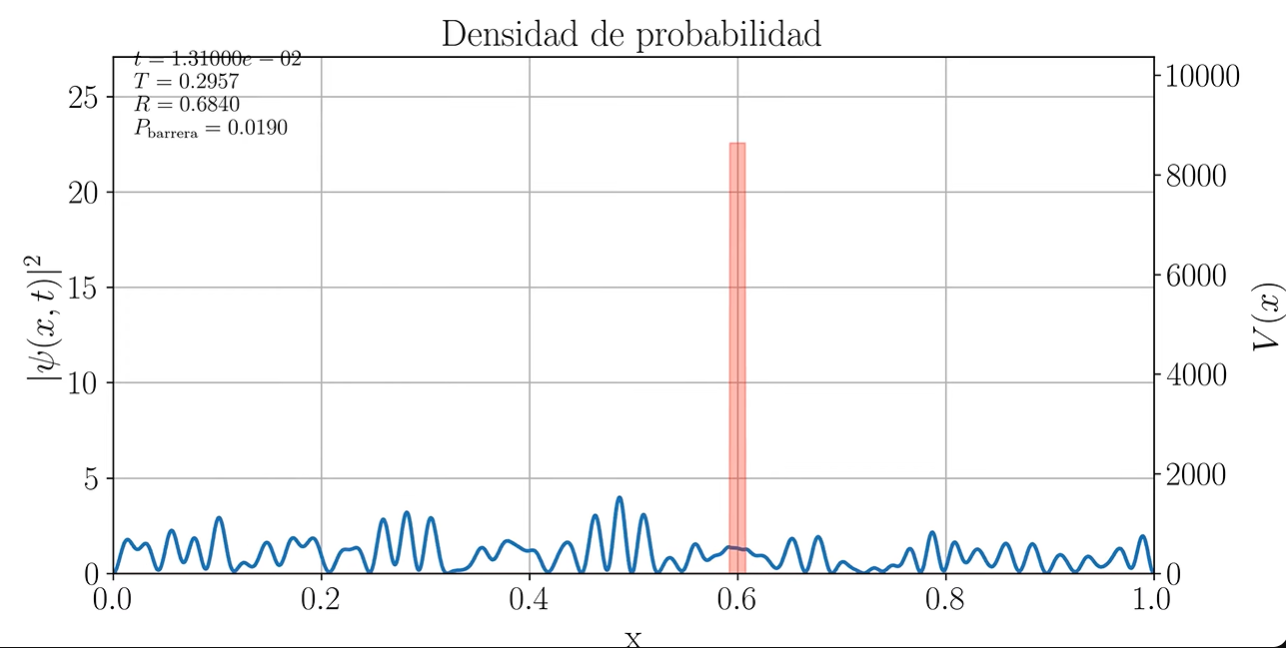
\includegraphics[width=0.75\linewidth]{figures/tunel_schrodinger.png}}
    \caption{Evolución temporal de la función de onda de un paquete gaussiano incidente sobre una barrera rectangular de potencial en el régimen \(V_0>E\). Animación completa disponible en \href{https://youtu.be/dDUh9E-eRjU}{YouTube}.}
    \label{fig:tunel_schrodinger}
\end{figure}


La simulación resuelve numéricamente la ecuación de Schrödinger unidimensional dependiente del tiempo mediante el esquema implícito de Crank–Nicolson. El sistema consiste en un paquete de ondas gaussiano inicialmente localizado en \(x_0=0.20\), propagándose con momento medio \(k_0=120\) hacia una barrera rectangular de altura \(V_0\) y anchura \(w\), centrada en \(x_c=0.60\).

La Figura \ref{fig:tunel_schrodinger} muestra la evolución temporal de la densidad de probabilidad \(|\psi(x,t)|^2\). Antes de alcanzar la barrera, el paquete mantiene una estructura gaussiana coherente y un perfil aproximadamente simétrico. Durante la interacción con la región potencial, la función de onda se divide dinámicamente en dos componentes: una fracción reflejada que se propaga hacia la izquierda y una fracción transmitida que emerge al otro lado de la barrera pese a verificarse el régimen clásico prohibido \(V_0>E\).

Por otro lado, la simulación registra la evolución temporal de las probabilidades integradas de transmisión \(T(t)\), reflexión \(R(t)\) y ocupación transitoria de la barrera \(P_{\mathrm{barrera}}(t)\). Los resultados constituyen una manifestación explícita del efecto túnel cuántico, fenómeno estrictamente prohibido en mecánica clásica.

Es decir, la atenuación que sufre la onda no implica la anulación completa de su amplitud, permitiendo una probabilidad finita de transmisión incluso en regiones clásicamente inaccesibles. Este comportamiento se ve reflejado en la Figura \ref{temporal} ya que la transmisión no permanece nula tras el primer encuentro de la onda con la barrera alrededor de $t\approx2.5\cdot10^{-3}s$, además, se verifica la estabilidad numérica del método debido a la conservación de la probabilidad dada por la Ecuación \ref{eq:conservacion_prob}. Este hecho comprueba que el algoritmo implementado respeta la unitariedad de la dinámica cuántica y valida el uso del método de Crank–Nicolson como herramienta robusta para estudiar fenómenos de transporte cuántico, dispersión resonante y propagación coherente en nanoestructuras potenciales.

\begin{figure}[H]
    \centering
    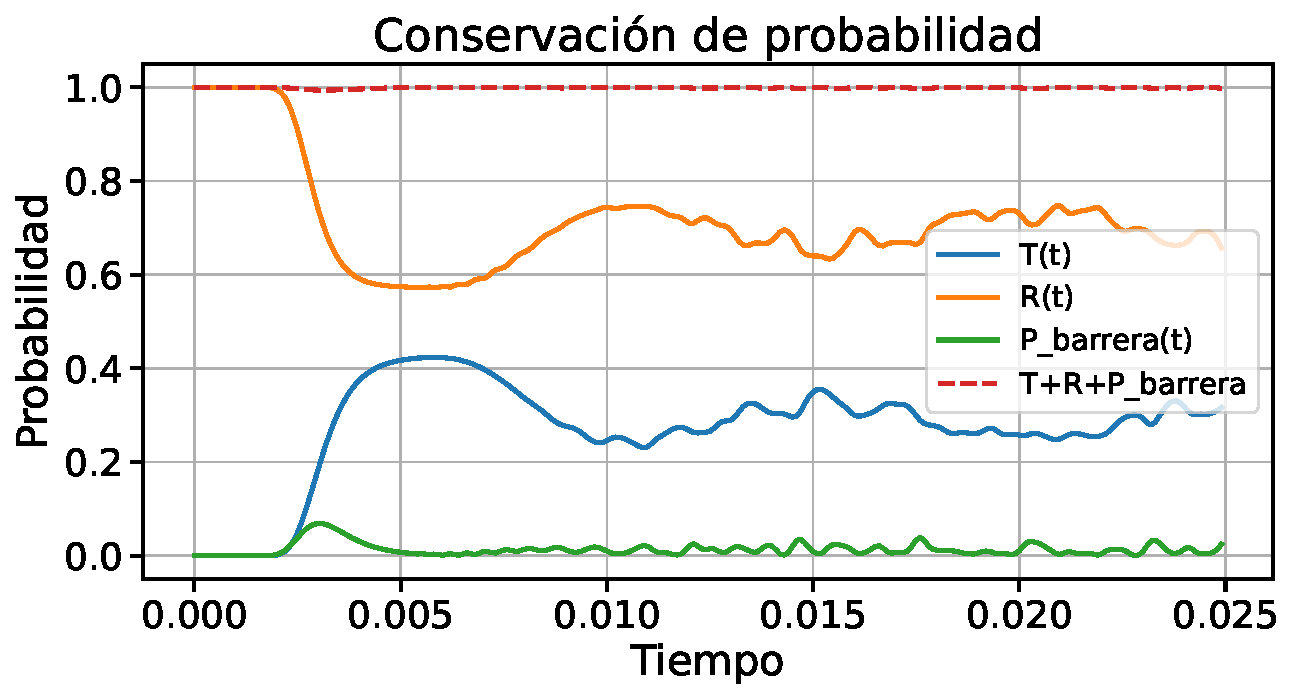
\includegraphics[width=0.7\textwidth]{figures/conservacion_probabilidad.pdf}
    \caption{Figura que muestra $R(t)$, $T(t)$, $P_{barrera}(t)$ así como $R(t)+T(t)+P_{barrera}(t)$.}
    \label{temporal}
\end{figure}

Por completitud, el primer pico de transmisión obtenido mediante Crank-Nicolson se puede comparar con la solución analítica, dada por la Expresión \ref{eq:T_analitica}, mostrando una similitud considerable en los resultados, con una desviación del 3\% ($T_{CN}^{max}=0.423,T_{an}=0.409)$. La correlación de estos resultados no es crítica para la veracidad de la simulación debido a que la fórmula analítica se obtiene en el caso de una onda plana que se propaga libremente hasta la barrera y tras atravesarla recupera su libertad de movimiento, pero su parecido sirve como una estimación para ratificar el buen funcionamiento del método.

Adicionalmente, se realizaron barridos paramétricos tanto en la altura del potencial \(V_0\) como en la anchura \(w\), obteniendo mapas bidimensionales \(T(V_0,t)\) y \(T(w,t)\), así como las transmisiones medias temporales \(\langle T \rangle\). Como se puede observar en la Figura \ref{fig:barridos}, el barrido paramétrico en $V_0$, evidencia que la transmisión decrece conforme aumenta la altura de la barrera, ya que el vector de decaimiento evanescente \(\kappa\) se incrementa y reduce la penetración efectiva de la función de onda. Por otro lado, el análisis respecto a la anchura \(w\) revela que pequeñas variaciones de grosor producen reducciones exponenciales de \(\langle T \rangle\). Este comportamiento reproduce directamente la predicción de la aproximación WKB, donde $T \sim e^{-2\kappa w}$.

\begin{figure}[H]
    \centering

    \begin{subfigure}[b]{0.42\textwidth}
        \centering
        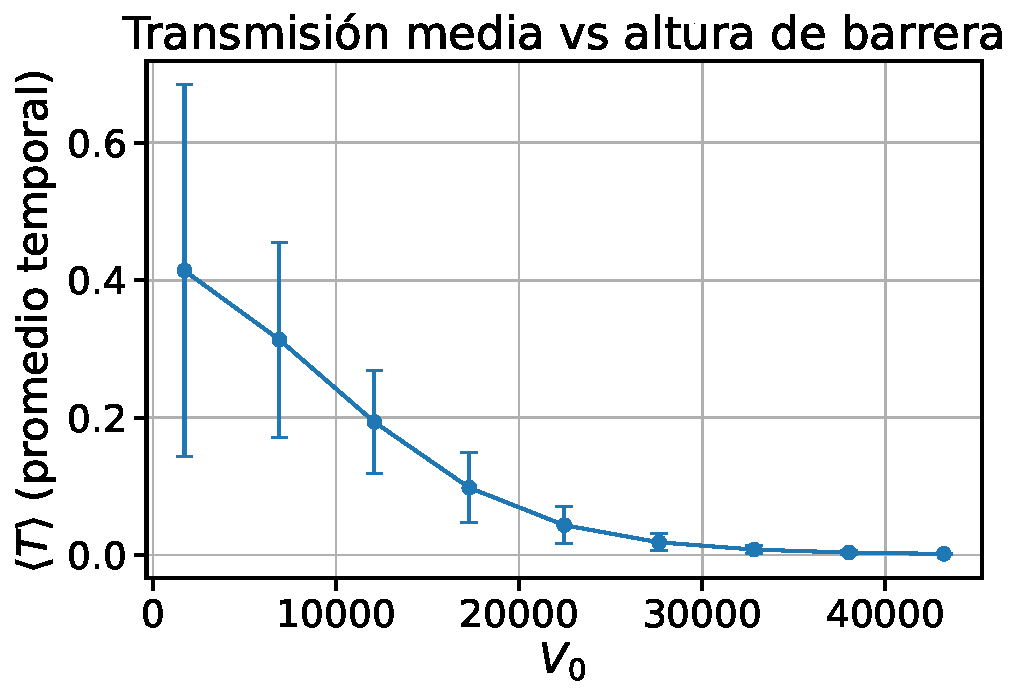
\includegraphics[width=\textwidth]{figures/T_medio_vs_V0.pdf}
        \caption{}
        \label{fig:barrido_V}
    \end{subfigure}
    \hfill
    \begin{subfigure}[b]{0.42\textwidth}
        \centering
        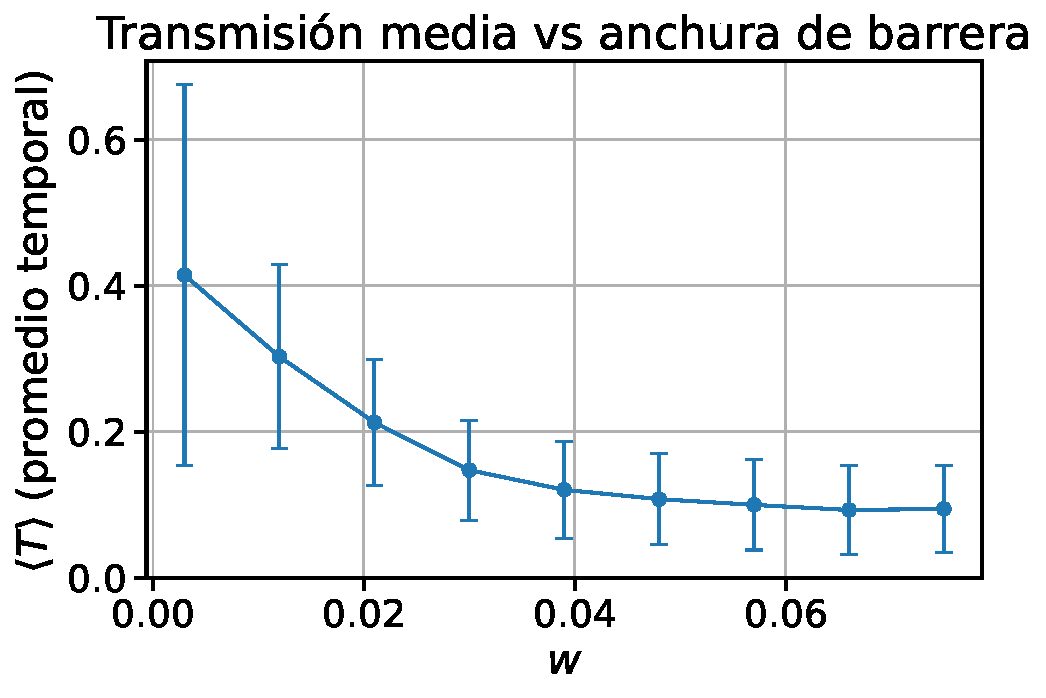
\includegraphics[width=\textwidth]{figures/T_medio_vs_w.pdf}
        \caption{}
        \label{fig:barrido_w}
    \end{subfigure}

    \caption{(a) Resultados del barrido para determinar $\langle T(V_0)\rangle_t$. (b) Resultados del barrido para determinar $\langle T(w)\rangle_t$}
  \label{fig:barridos}
\end{figure}

Otra forma de visualizar estos mismos resultados es un mapa que muestra $T(V_0,t)$ y $T(w,t)$, como se observa en la Figura \ref{fig:mapas}.

\begin{figure}[H]
    \centering

    \begin{subfigure}[b]{0.48\textwidth}
        \centering        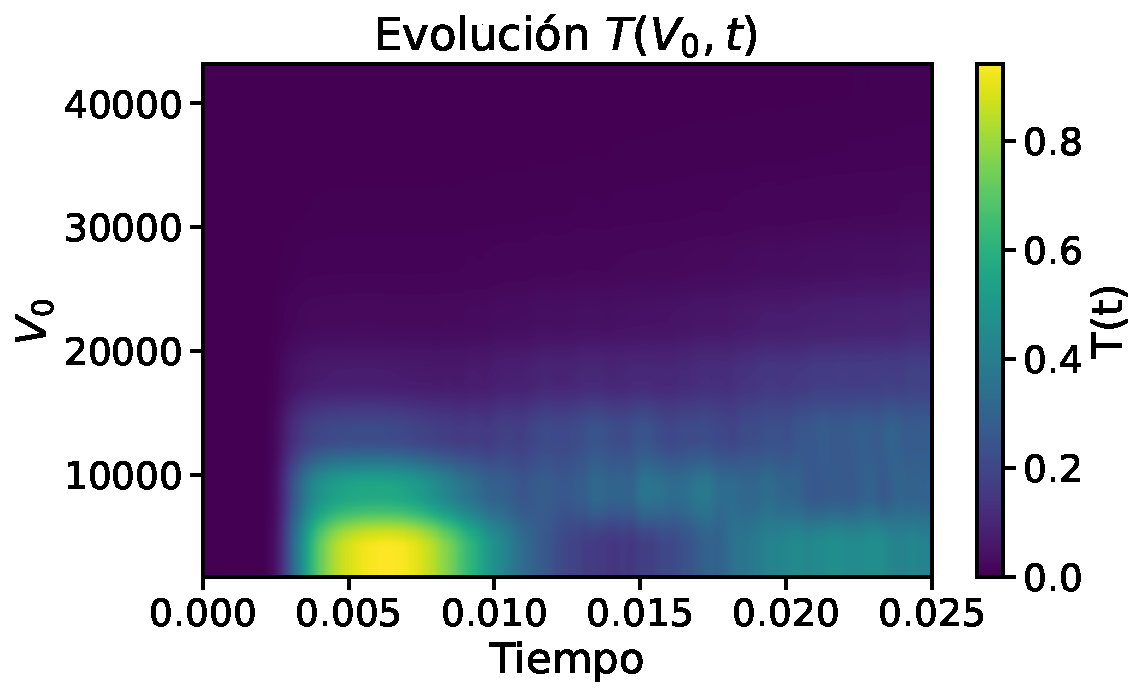
\includegraphics[width=\textwidth]{figures/mapa_T_V0.pdf}
        \caption{Evolución $T(V_0,t)$}
        \label{fig:mapa_V}
    \end{subfigure}
    \hfill
    \begin{subfigure}[b]{0.48\textwidth}
        \centering
        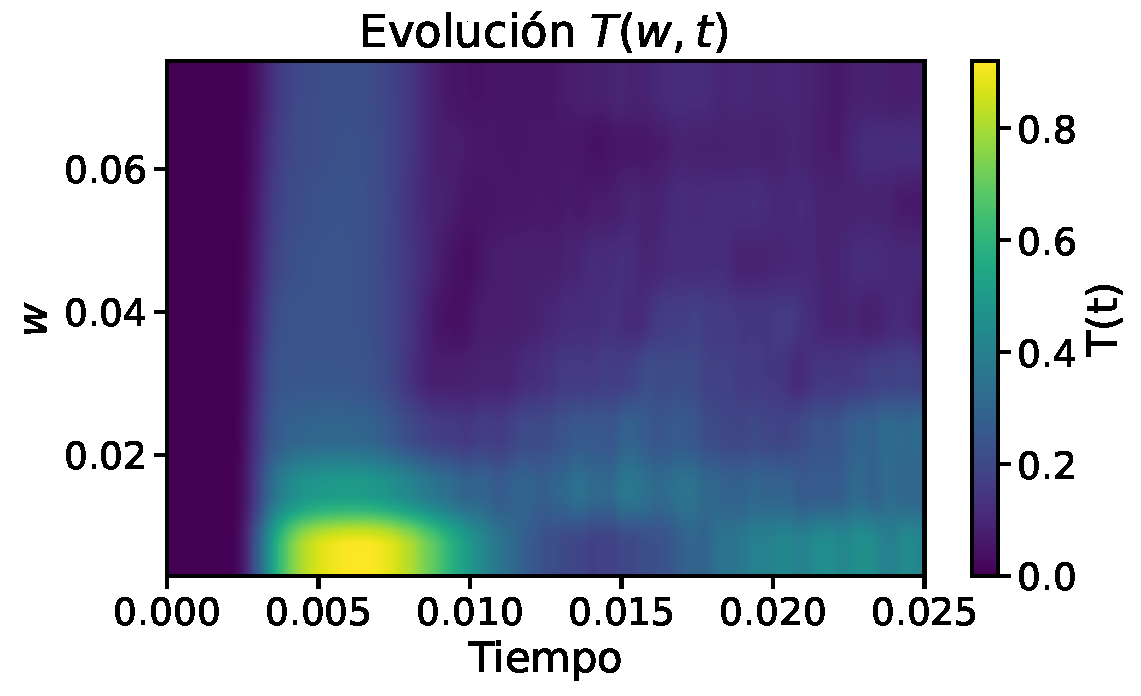
\includegraphics[width=\textwidth]{figures/mapa_T_w.pdf}
        \caption{Evolución $T(V_0,t)$}
        \label{fig:mapa_w}
    \end{subfigure}

    \caption{Mapas 2D que muestran la evolución de la probabilidad de transmisión $T$ en función del tiempo variando $V_0$ (Izquierda) o $w$ (Derecha).}
  \label{fig:mapas}
\end{figure}

Finalmente, la animación de la parte real \(\Re(\psi)\) (Figura \ref{fig:real_part}) muestra la conservación de coherencia de fase durante todo el proceso de dispersión. Las oscilaciones espaciales preservan continuidad incluso tras la separación entre componentes transmitidas y reflejadas, evidenciando que el fenómeno de túnel no puede interpretarse como una transición clásica estocástica, sino como la evolución determinista de un estado cuántico coherente distribuido espacialmente.


\begin{figure}[h!]
    \centering
    \href{https://youtu.be/frQ7Apgdps4}{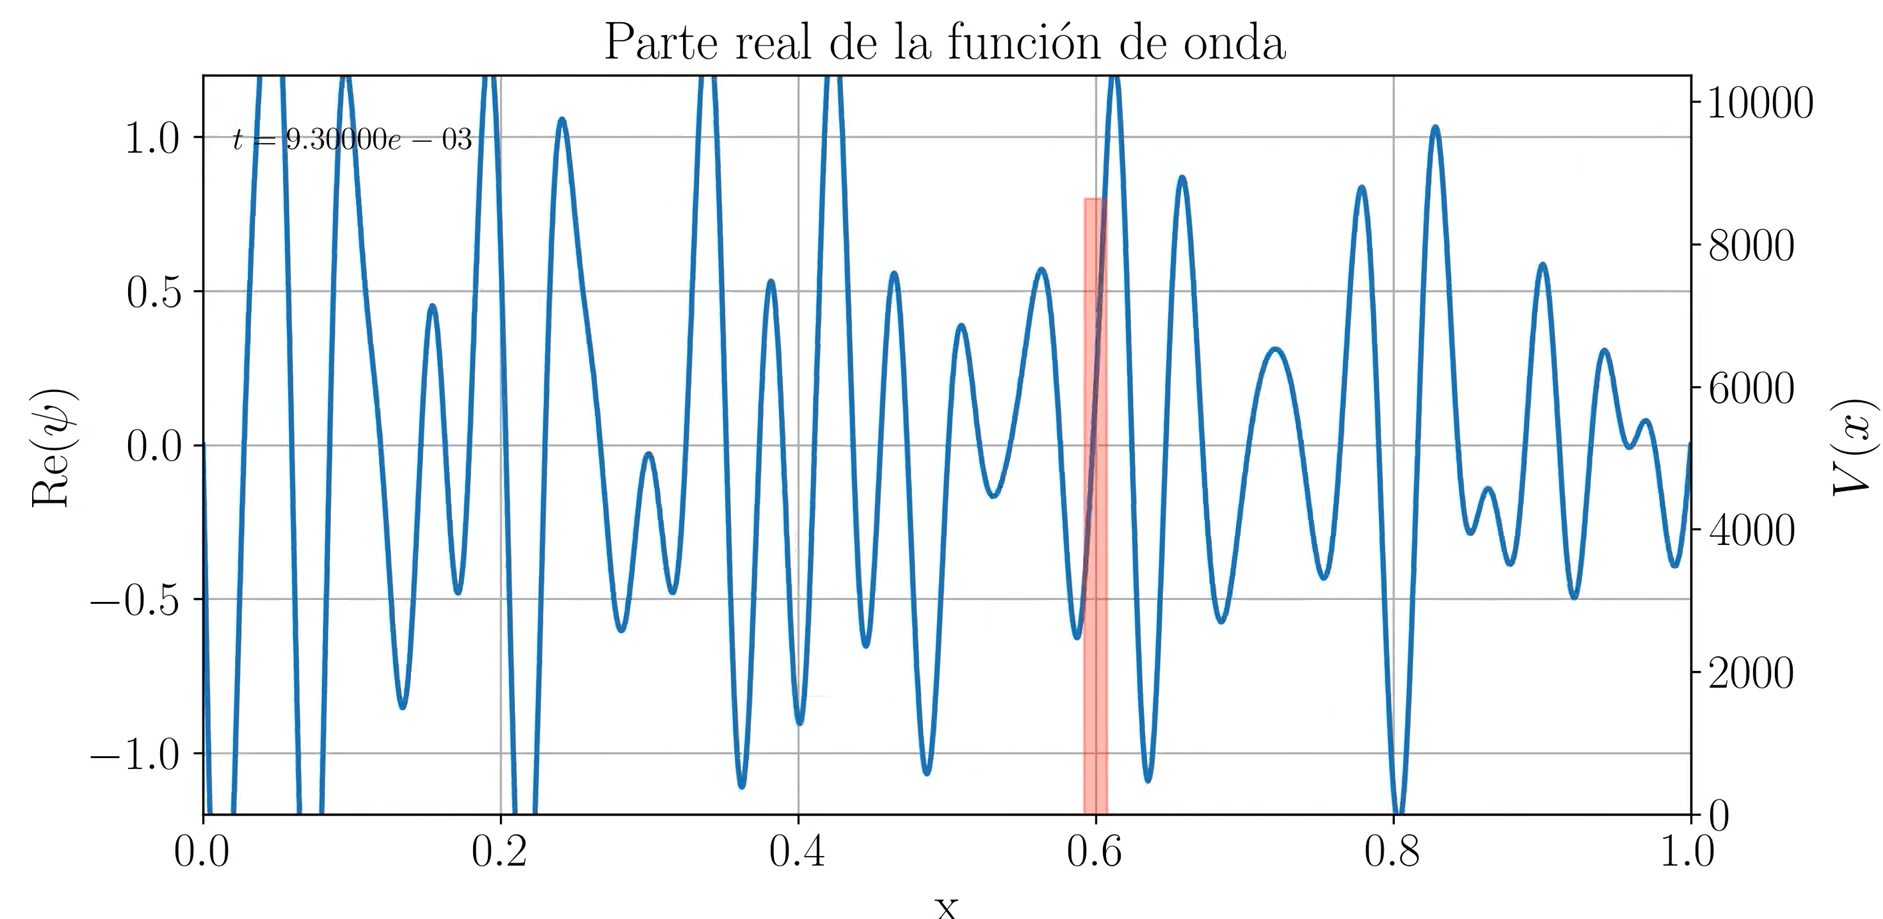
\includegraphics[width=0.75\linewidth]{figures/real_part.png}}
    \caption{Evolución temporal de la parte temporal un paquete gaussiano incidente sobre una barrera rectangular de potencial en el régimen $V_0>E$. Animación completa disponible en \href{https://youtu.be/frQ7Apgdps4}{YouTube}.}
    \label{fig:real_part}
\end{figure}

% ---------------------------------------------------------
% 1. Experimento de Doble Rendija
% ---------------------------------------------------------


\subsection{Resultados y Análisis: Simulación de Doble Rendija}

La visualización temporal detalla la evolución de un paquete de ondas incidente que se propaga hacia un obstáculo situado en $x = 0 $. Antes de la colisión (zonas de $x \approx -20 \, a_0$), la función de onda exhibe un frente de fase coherente. Al atravesar las rendijas, el haz experimenta difracción radial, conformando un patrón de franjas de interferencia. La escala cromática parametriza la fase (o argumento) de la función de onda compleja, variando estrictamente en el dominio $\arg(\psi) \in [-\pi, \pi]$.


\begin{figure}[h!]
    \centering
    \href{https://youtube.com/shorts/XPvwuIbuQ5A?feature=share}{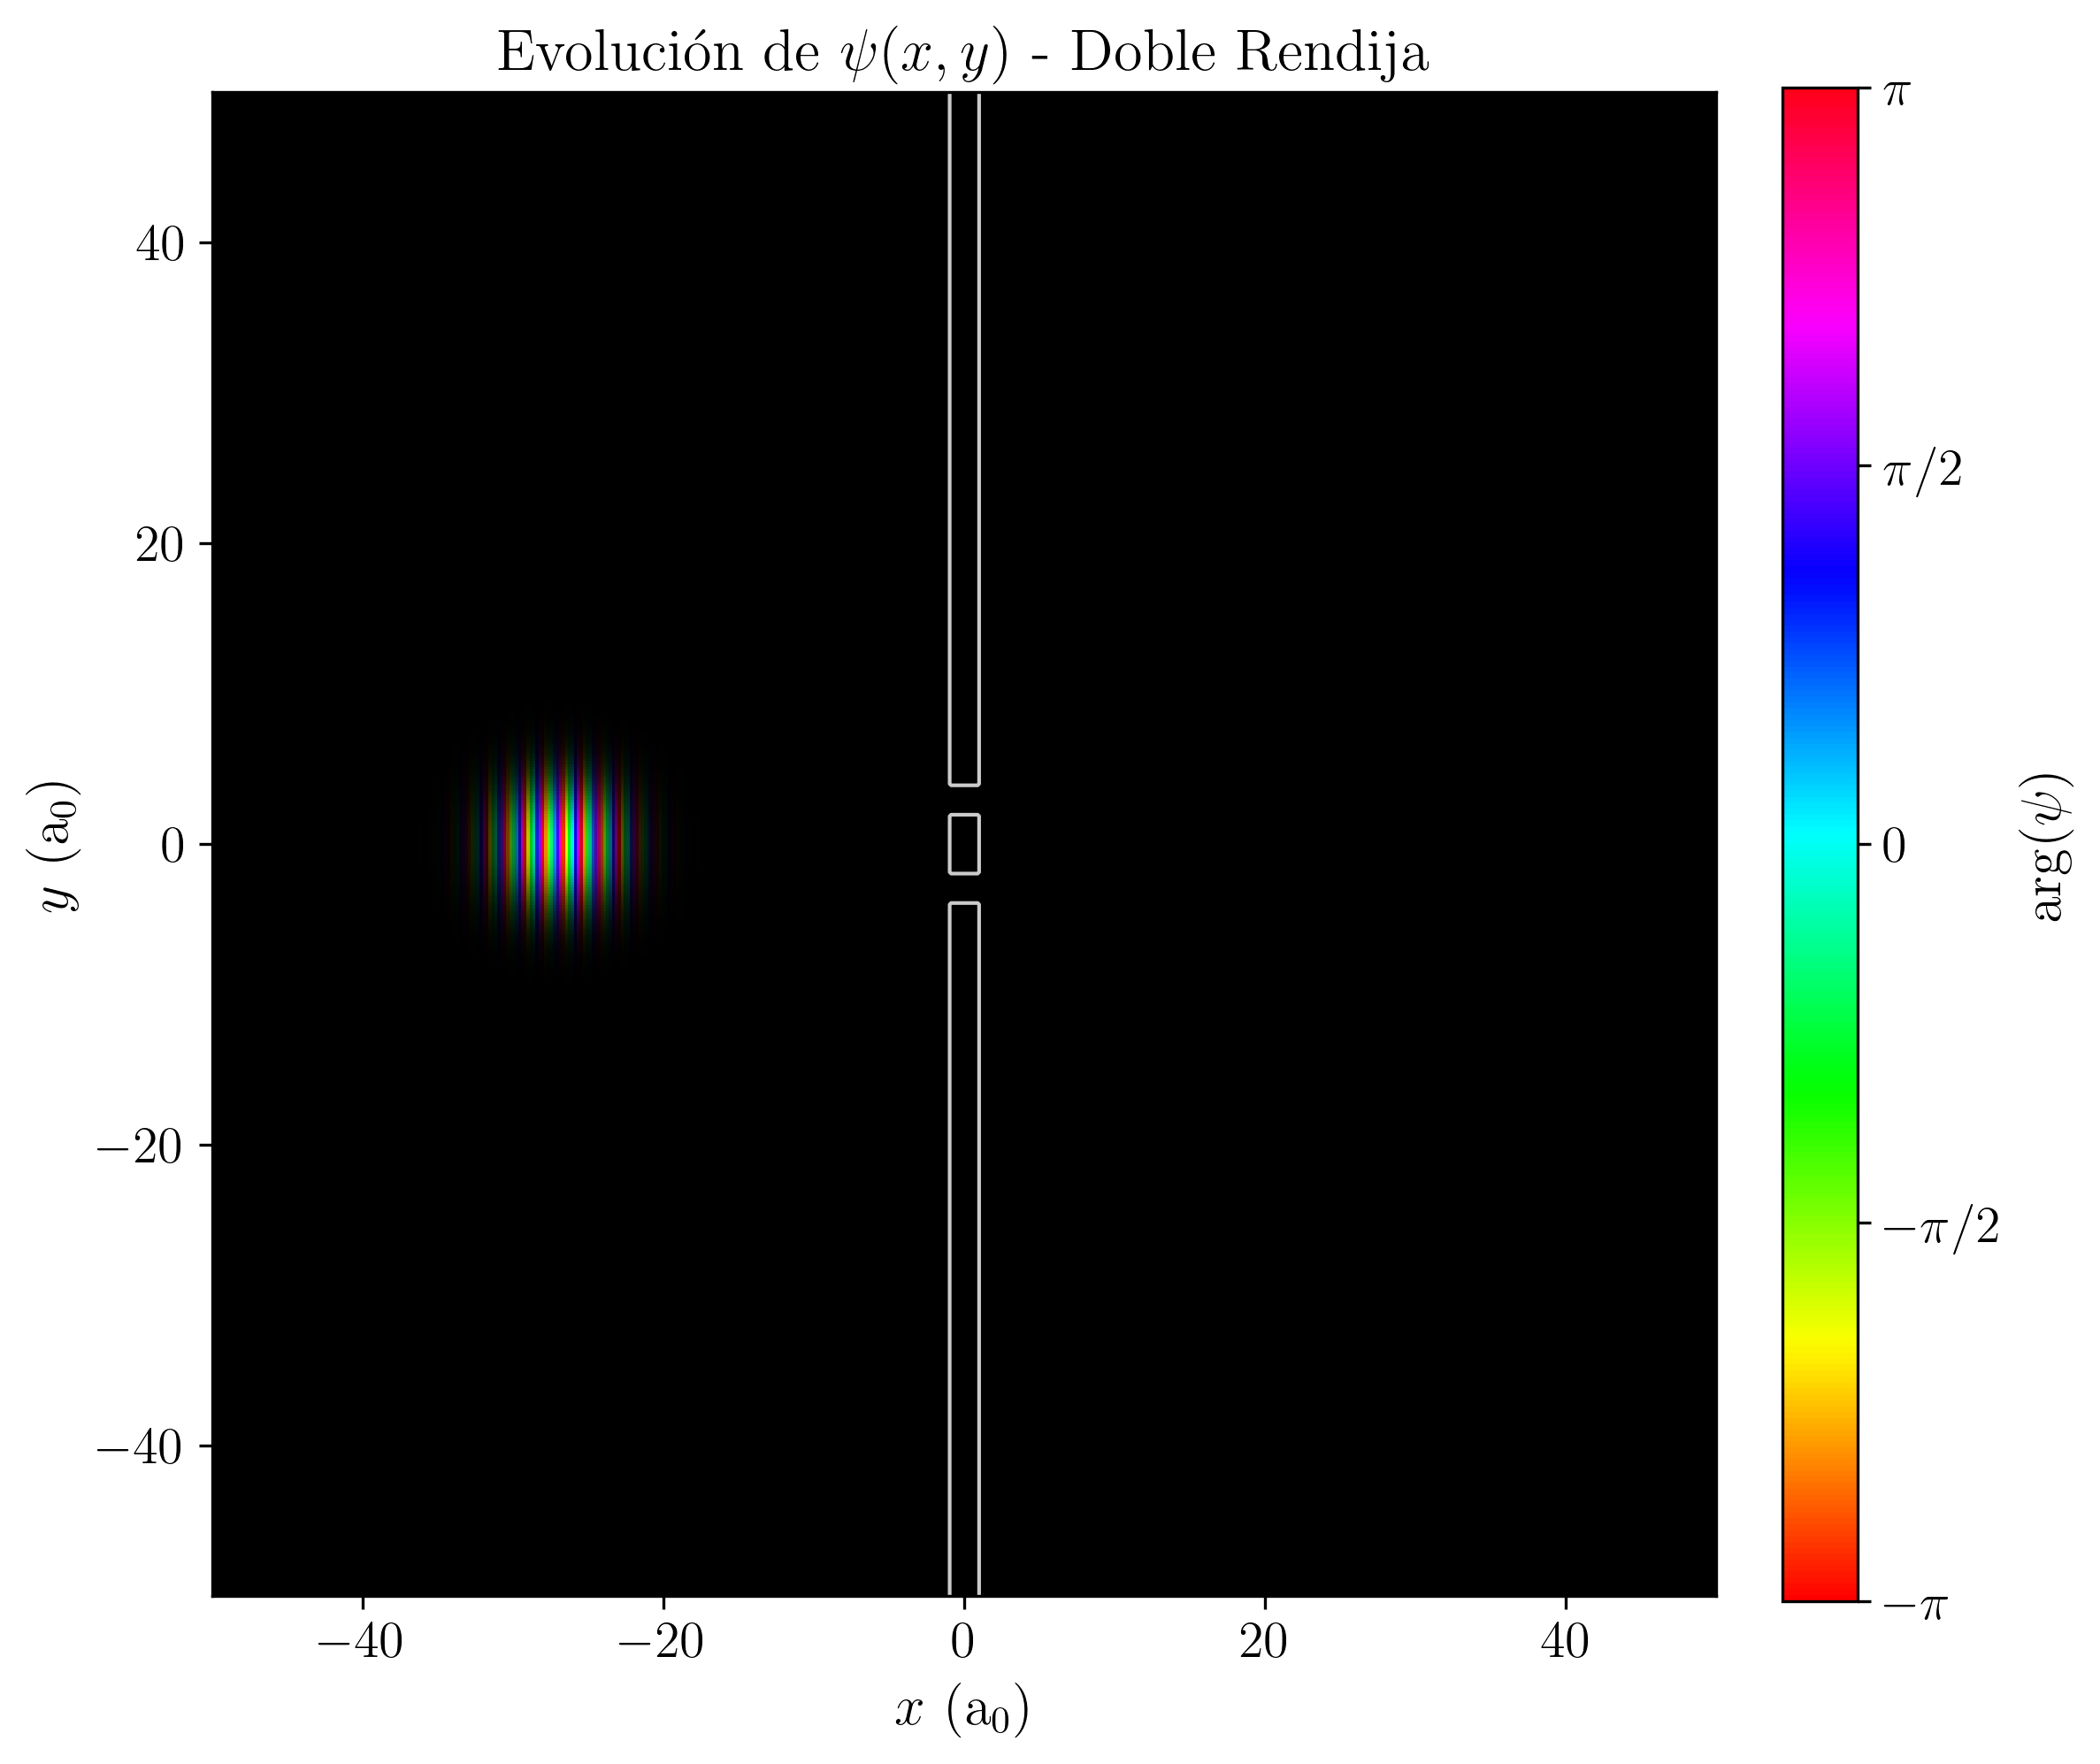
\includegraphics[width=0.65\linewidth]{figures/doble_rendija.png}}
    \caption{Experimento de la Doble Rendija. Animación completa en \href{https://youtube.com/shorts/XPvwuIbuQ5A?feature=share}{YouTube}}
\end{figure}

El comportamiento espaciotemporal registrado es una manifestación fenomenológica explícita de la ecuación de Schrödinger dependiente del tiempo. La emergencia de un patrón de franjas posterior a $x = 0 $ confirma la naturaleza ondulatoria y el principio de superposición cuántica. Las transiciones topológicas de coloración (de $-\pi$ a $\pi$) acopladas a nodos de amplitud nula revelan la interferencia destructiva, lo cual atestigua la conservación de la coherencia de fase del estado cuántico tras la bipartición espacial del haz original.

% ---------------------------------------------------------
% 2. Estructura Atómica del Nanografeno
% ---------------------------------------------------------

\subsection{Resultados y Análisis: Difracción de Nanografeno (HBC)}

A continuación, se presentan y analizan los resultados obtenidos de la simulación numérica del experimento de difracción de campo lejano utilizando moléculas de nanografeno (Hexa-peri-benzocoroneno, HBC) como frentes de onda coherentes. El análisis abarca desde la caracterización de la estructura de la muestra en el espacio real hasta la interpretación de los patrones de interferencia resultantes.

\subsubsection{Caracterización de la Muestra en el Espacio Real}
La Figura \ref{fig:estructura_hbc} proporciona un mapeo coordenado detallando la arquitectura atómica del nanografeno (HBC) utilizado como rejilla de difracción. A diferencia de un conglomerado de moléculas aisladas, este clúster molecular se compone de una red densa de siete anillos hexagonales aromáticos fusionados, donde los anillos periféricos comparten enlaces carbono-carbono con el anillo central.

\begin{figure}[h!]
    \centering
    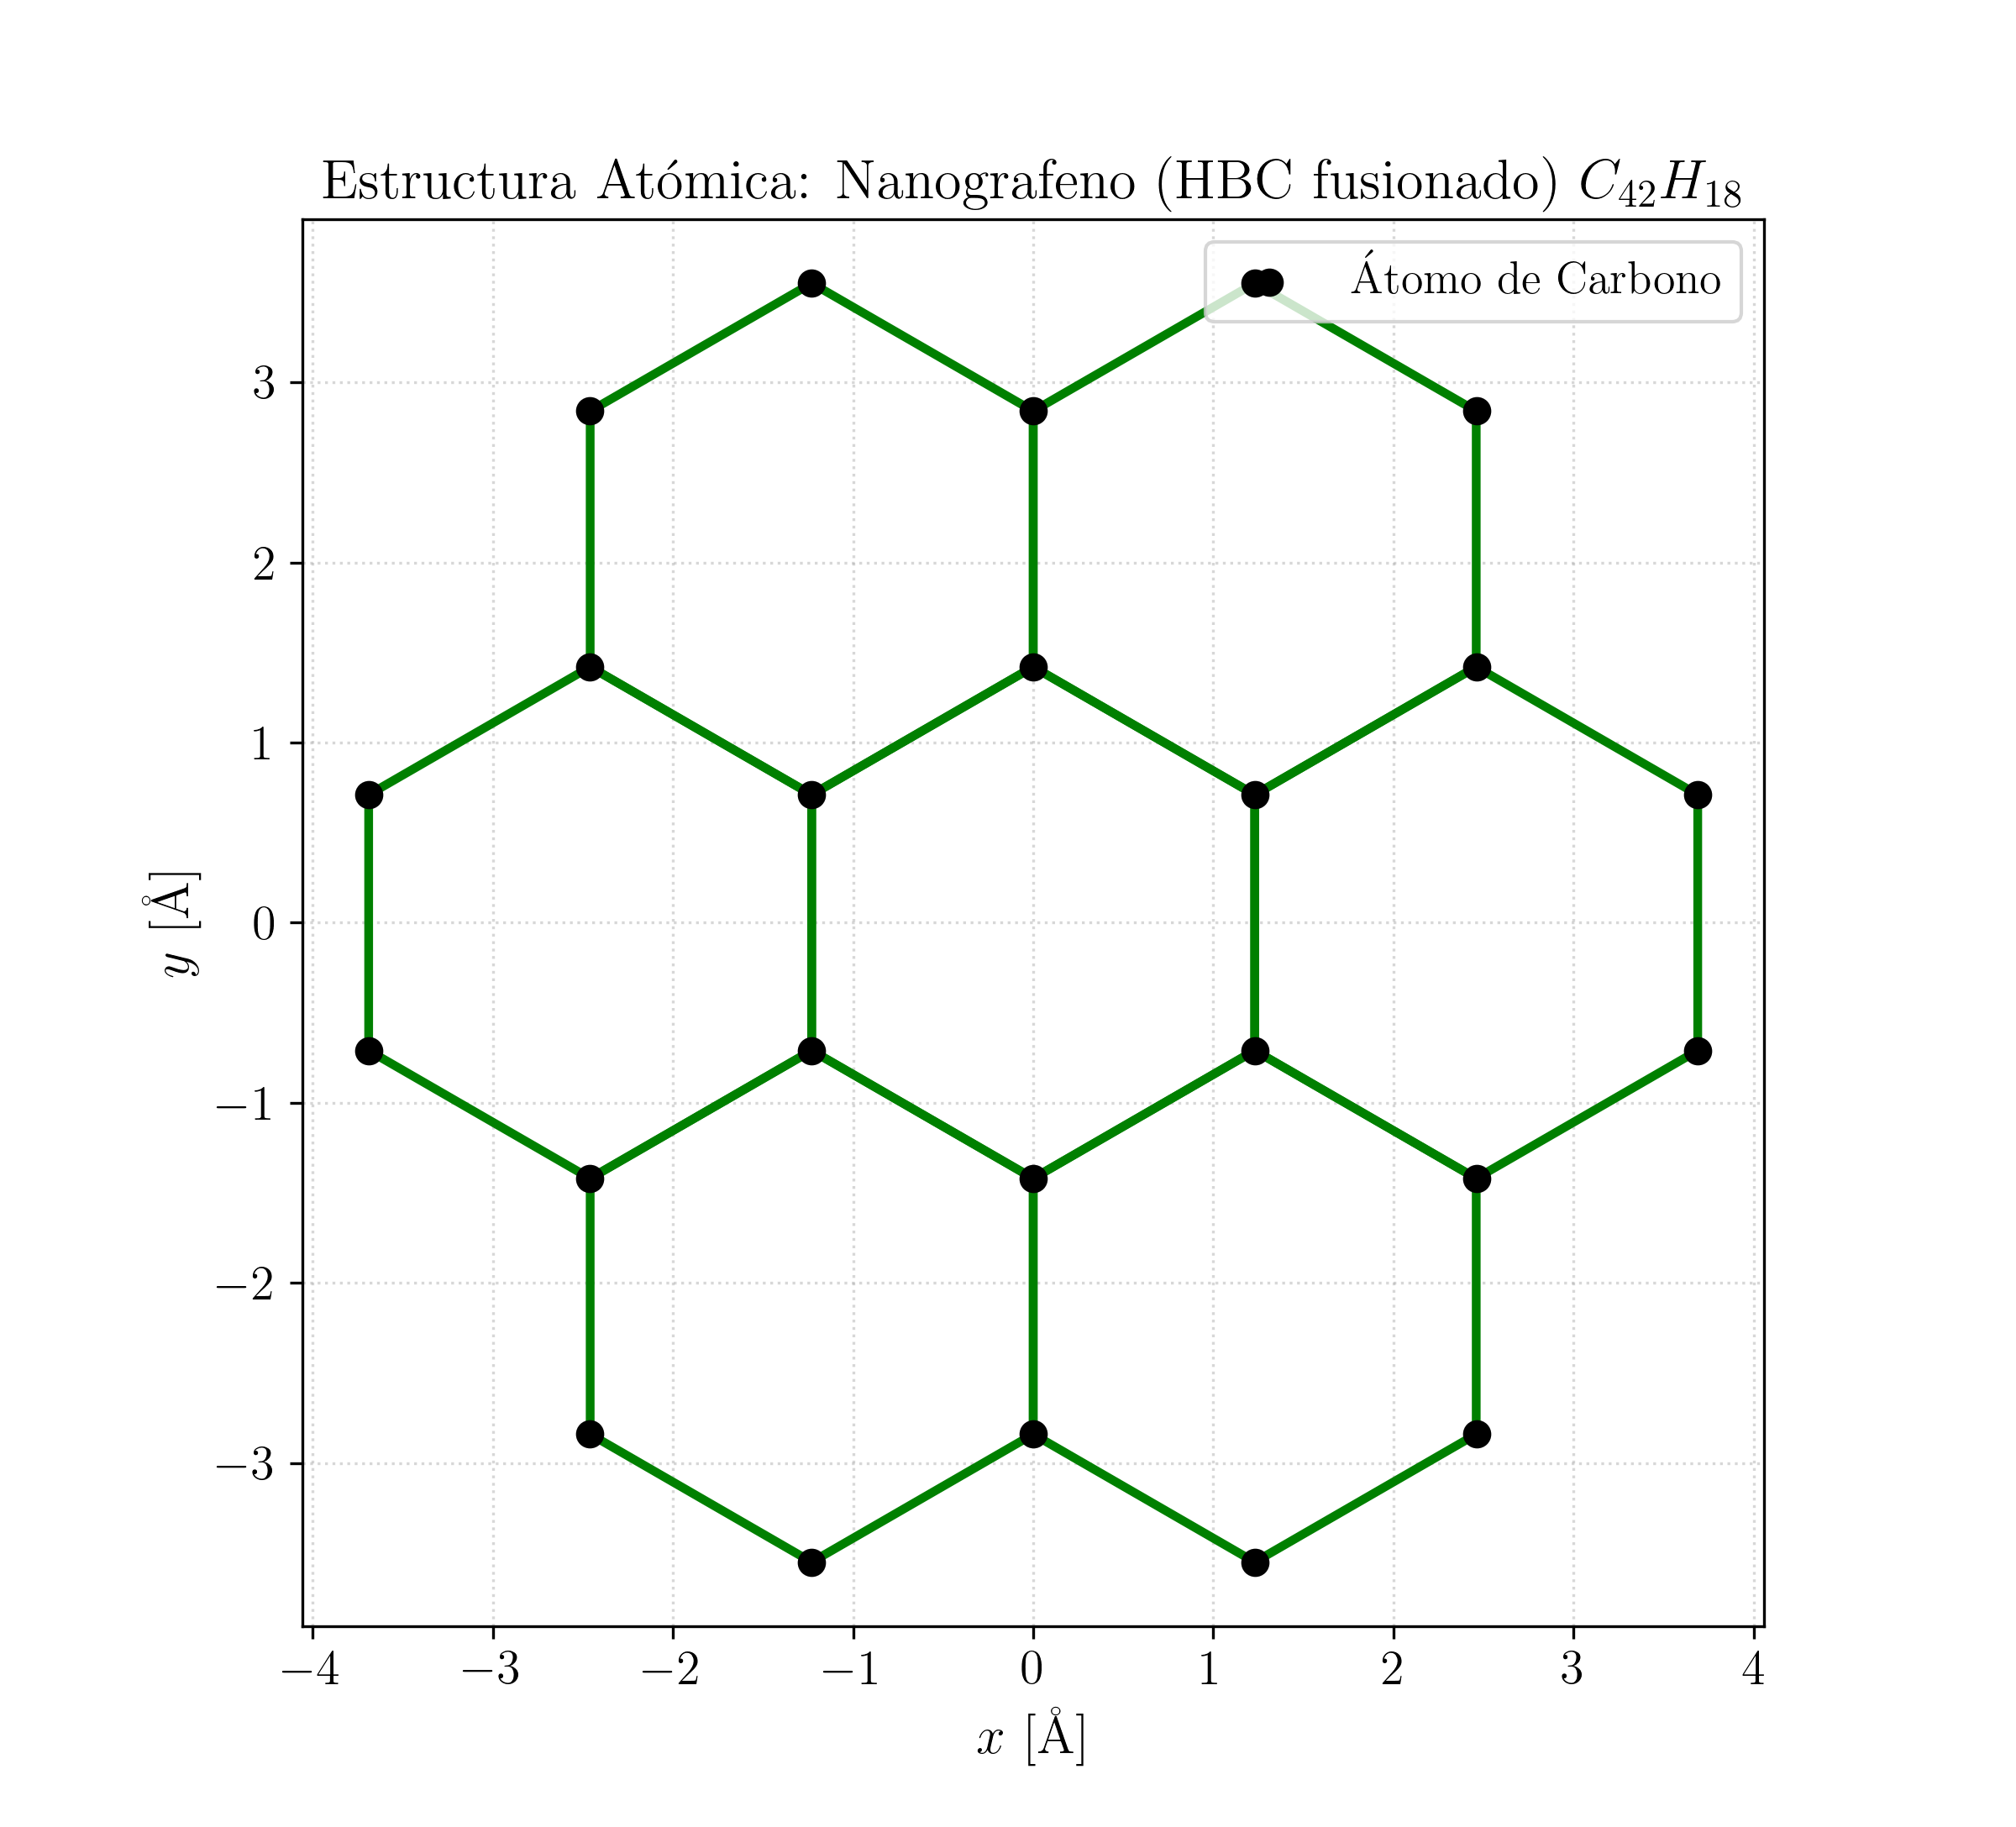
\includegraphics[width=0.5\textwidth]{figures/estructura_atomica_nanografeno_fused.png}
    \caption{Disposición geométrica fusionada de la red en el espacio real para la molécula de Hexa-peri-benzocoroneno ($C_{42}H_{18}$). Los puntos negros representan los 42 átomos de carbono únicos y las líneas verdes los enlaces covalentes compartidos.}
    \label{fig:estructura_hbc}
\end{figure}

Las coordenadas están proyectadas en unidades de angstroms (\AA) para ambos ejes. El entramado atómico se extiende en una región espacial de aproximadamente $-5 \, \text{\AA}$ a $5 \, \text{\AA}$ en el eje transversal ($x$) y de $-5 \, \text{\AA}$ a $5 \, \text{\AA}$ en el eje vertical ($y$), evidenciando una distancia de enlace C-C consistente de $1.42 \, \text{\AA}$ en toda la topología fusionada.

% La estricta periodicidad hexagonal y la naturaleza fusionada de los anillos manifiestan la hibridación orbital $sp^2$ intrínseca de los sistemas aromáticos policíclicos de carbono. Esta macro-molécula plana exhibe un grupo de simetría puntual $D_{6h}$. Identificar con alta precisión este arreglo espacial y su densidad electrónica $\rho(\mathbf{r})$ es un prerrequisito analítico fundamental, ya que su Transformada de Fourier dictaminará las direcciones permitidas de dispersión constructiva en el espacio recíproco.

% ------------------------------------------------------------------------------
% SUB-SUBSECCIÓN: DINÁMICA DE PROPAGACIÓN
% ------------------------------------------------------------------------------
\subsubsection{Dinámica de Propagación y Acumulación de Intensidad}

La visualización de la dinámica de las moléculas desde la rejilla hasta la pantalla se presenta mediante una animación (Figura \ref{fig:animation_scat}).



\begin{figure}[H]
    \centering
\href{https://youtu.be/2b96mZdyjBI}{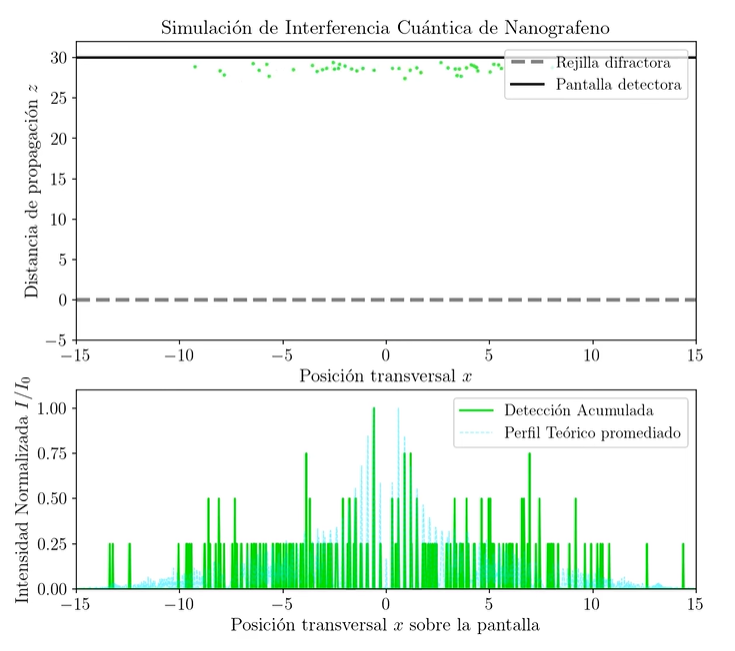
\includegraphics[width=0.7\linewidth]{figures/animation_thumbnail.png}}
    \caption{Instantánea de la animación de simulación. Panel superior: Propagación de las moléculas (puntos verdes) en el espacio $x-z$. El panel inferior muestra la evolución del histograma de detección transversal ($I/I_0$) en la pantalla ($z=30$) a medida que se acumulan eventos. Animación disponible en \href{https://youtu.be/dHB0DgZWk-c}{YouTube}.}
    \label{fig:animation_scat}
\end{figure}

La interfaz de resultados muestra dos paneles acoplados temporalmente. El panel superior constata la propagación longitudinal de las moléculas a lo largo del eje $z$, desde la rejilla difractora ($z=0$) hasta la pantalla situada en $z = 30$, mostrando la expansión transversal del haz. Paralelamente, el panel inferior reporta el perfil de intensidad relativa ($I/I_0$) en función de la coordenada transversal $x \in [-15, 15]$. Se identifica un pico principal o lóbulo central en $x = 0$ con convergencia máxima de $I/I_0 = 1.0$, flanqueado por picos secundarios sinusoidales amortiguados. Se observa un solapamiento casi directo entre la curva de la ``Detección Acumulada'' (puntos muestreados aleatoriamente) y el ``Perfil Teórico promediado'' (curva cian).

La máxima amplitud registrada en el origen corresponde al orden de difracción $0$, representativo del volumen de la onda no dispersada. Las oscilaciones paramétricas colindantes son el resultado directo de la interferencia constructiva de múltiples rendijas (factor de estructura) impuesta por la red atómica de la muestra de HBC. La convergencia del histograma de partículas hacia el modelo teórico certifica la validez estadística de la simulación de Monte Carlo y confirma que el montaje operó bajo condiciones de alta coherencia longitudinal, permitiendo la resolución de picos de interferencia de alto orden.

% ------------------------------------------------------------------------------
% SUB-SUBSECCIÓN: PATRÓN 2D
% ------------------------------------------------------------------------------
\subsubsection{Mapeo del Patrón de Interferencia Bidimensional}

Para examinar la simetría del patrón de difracción en todo el plano de detección, se generó un mapeo bidimensional de intensidad (Figura \ref{fig:patron_2d}).

\begin{figure}[h]
    \centering
    % Se asume que el archivo '2d_pattern_graphene.png' está en la carpeta 'figures'
    % Este es el nombre exacto generado por el código corregido.
    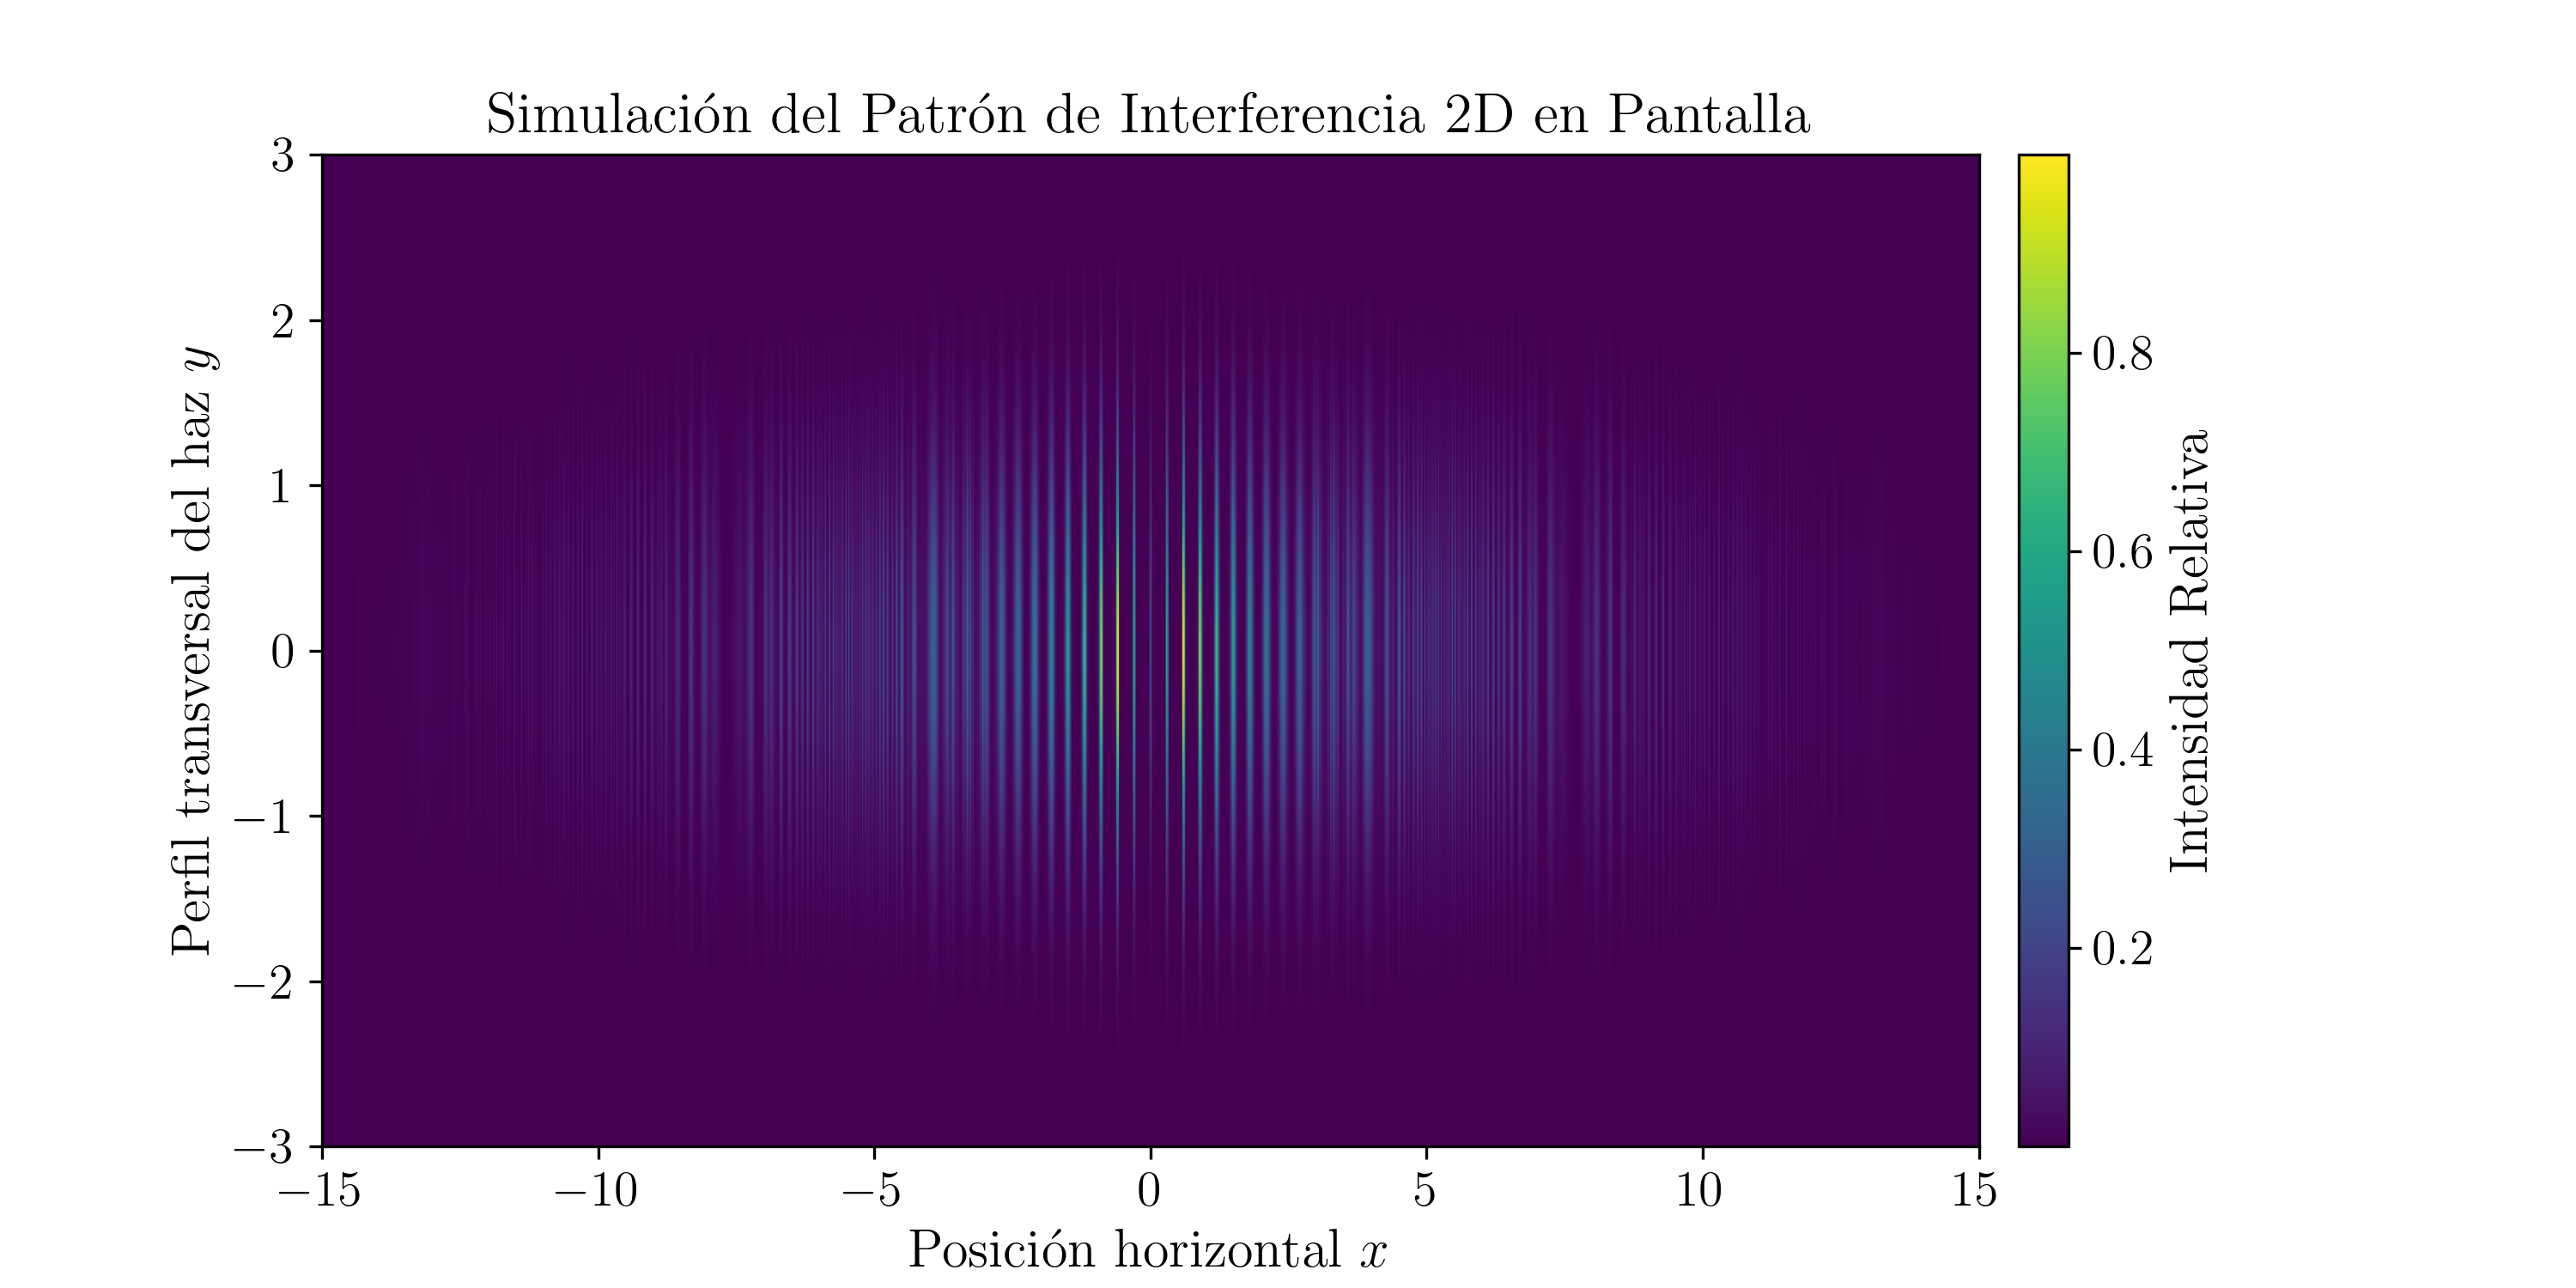
\includegraphics[width=1\textwidth]{figures/2d_pattern_graphene.png}
    \caption{Mapeo bidimensional de intensidad (mapa de calor usando escala 'viridis') para el campo de interferencia de la estructura de nanografeno en la pantalla de detección.}
    \label{fig:patron_2d}
\end{figure}

El gráfico es un mapa de calor  que representa la Intensidad Relativa de Interferencia. Se define el dominio espacial con la Posición horizontal $x \in [-15, 15]$ en el eje de abscisas, cruzada con el Perfil transversal del haz $y \in [-3, 3]$ en las ordenadas. La métrica de color evalúa la intensidad, mostrando una topografía de franjas de difracción verticales densamente empaquetadas. Debido a la envolvente gaussiana simulada en el eje Y para modelar el perfil limitado del haz incidente, la intensidad alcanza sus picos locales máximos en el centro de masa del patrón ($y \approx 0, x \approx 0$), degradándose paulatinamente hacia los bordes periféricos verticales.

Esta visualización codifica la sección eficaz de dispersión coherente mapeada sobre un plano de detección bidimensional en el régimen de Fraunhofer. La marcada anisotropía del patrón (franjas orientadas longitudinalmente) constituye la huella espectral de las restricciones de simetría de la red de HBC fusionado analizada en la Figura \ref{fig:estructura_hbc}. 
% Los máximos de intensidad delimitan los ángulos sólidos que satisfacen la condición de interferencia constructiva de Bragg-Laue, confirmando que la función de onda de prueba fue sensible al arreglo atómico periódico en la escala nanométrica.

% En el dominio 2D, el experimento exhibe visualmente la auto-interferencia macromolecular: el frente de onda continuo se fractura formando lóbulos con fases intercaladas en el eje X, modulados por la intensidad del haz en el eje Y, y separados por líneas nodales de interferencia destructiva estricta.

% Finalmente, la integración del espectro térmico (policromaticidad) en la simulación del nanografeno modela fielmente la realidad experimental. Se constata que la macromolécula actúa como un frente de onda coherente; sin embargo, la dispersión de velocidades provoca que los diferentes regímenes de difracción asociados a cada longitud de onda de de Broglie se solapen. Como resultado visual, el lóbulo central (orden cero) preserva su nitidez geométrica, mientras que los picos de interferencia de orden superior sufren un emborronamiento progresivo hasta fundirse en un continuo incoherente, ratificando la extrema sensibilidad de los sistemas macromoleculares a su entorno térmico longitudinal.
\section{Conclusiones Generales}

A partir del análisis sistemático y secuencial de las simulaciones fundamentales y los datos de dispersión molecular, se extraen las siguientes conclusiones integrales que abarcan todos los fenómenos estudiados:

\textbf{Efecto Túnel y Validación Numérica:} La simulación Crank-Nicolson 1D reproduce con alta precisión la transmisión para una barrera rectangular con $V_0 > E$. El barrido paramétrico confirma que $T$ decrece $V_0$ y $w$, en concordancia con la  aproximación WKB. Por otro lado, la conservación de probabilidad $T+R+P_\text{barrera}\approx 1$ durante toda la evolución atestigua la estabilidad y fiabilidad del esquema implícito empleado.
 
\textbf{Dinámica Cuántica en la Doble Rendija:} La evolución espaciotemporal de la función de onda $\psi(x,y)$ demuestra fenomenológicamente el principio de superposición cuántica. La división topológica del paquete de ondas incidente genera dos frentes de onda coherentes que interactúan, formando un patrón de interferencia determinista. Las transiciones de fase ($\arg(\psi) \in [-\pi, \pi]$) evidencian que el sistema conserva la coherencia de fase global durante la propagación, validando de forma visual las predicciones de la ecuación de Schrödinger dependiente del tiempo para la difracción de materia pura.


\textbf{Precisión de la Simulación de Monte Carlo:} El análisis cuantitativo del perfil transversal de intensidades ($I/I_0$) constata una convergencia excepcional entre la detección acumulada de partículas y el modelo teórico policromático promediado. La morfología del pico central (orden cero) y las oscilaciones secundarias adyacentes certifican que el factor de estructura asociado a la periodicidad atómica del HBC y el factor de forma de las rendijas fueron parametrizados correctamente, evidenciando un evento de difracción macromolecular coherente.


La concatenación de estos resultados establece un puente directo entre los principios fundamentales de la interferencia (doble rendija) y sus aplicaciones cristalográficas avanzadas (nanografeno). Queda demostrado empírica y teóricamente que la difracción de materia coherente constituye un método analítico riguroso y no destructivo, capaz de trasladar las propiedades geométricas microscópicas al espacio recíproco para la caracterización precisa de materiales bidimensionales complejos.









%%%%%%%%%%%%%%%%%%%%%%%%%%%%%%%%%%
\bibliography{biblio}
\nocite{*}
\end{document}